\documentclass[10pt,a4paper]{article}
\usepackage[utf8]{inputenc}
\usepackage{ae}
\usepackage[brazil]{babel}
\usepackage[vmargin=2cm,hmargin=2cm,columnsep=0.75cm]{geometry}
\usepackage{float,nonfloat}
\usepackage{graphicx,color}
\usepackage{subcaption}
\usepackage{amsmath}

\makeatletter
\let\@institution\empty
\def\institution#1{\def\@institution{#1}}
\renewcommand{\maketitle}{
    \begin{center}
        {\Large\bfseries\@title\par\medskip}
        {\large
            \begin{tabular}[t]{c}%
                \@author
        \end{tabular}\par\medskip}
        {\itshape\@institution\par}
        {\itshape\@date\par}
\end{center}}
\makeatother

\newcommand{\pixel}{\textit{pixel} }
\newcommand{\pixels}{\textit{pixels} }

\begin{document}
% ============================================================================

\title{MC920: Introdução ao Processamento de Imagem Digital\\Tarefa 3}
\author{
    \begin{minipage}{6cm}
        \centering
        Martin Ichilevici de Oliveira\\
        RA 118077
    \end{minipage}
    \and
    \begin{minipage}{6cm}
        \centering
        Rafael Almeida Erthal Hermano\\
        RA 121286
    \end{minipage}
}
\institution{Instituto de Computação, Universidade Estadual de Campinas}
\date{\today}

\maketitle

% ============================================================================


\section{Casamento de histogramas}
Uma forma de modificar as intensidades de uma imagem é casando o seu histograma com o de outra. Esta transformação faz com que uma imagem fique com o histograma mais parecido possível com de outra imagem. Esta técnica pode ser utilizada para melhorias de brilho e contraste de uma imagem baseado em uma imagem de referência.

Sejam $f: A^2\rightarrow A$ e $g : A^2 \rightarrow A | A \subset N$, duas imagens em tons de cinza, e $T_1$ e $T_2$ transformações de equalização para $f$ e $g$ respectivamente. Para realizar o casamento de histogramas de $f$ em $g$, devemos aplicar a inversa de $T_2$ na equalização $T_1$.

Casamento = $T_2^{-1}(T_1(f))$

Aplicou-se o casamento histogrâmico conforme mostra a Figura \ref{fig:cas_hist}. A Figura \ref{fig:src} serviu como referência para o histograma, e a Figura \ref{fig:dst} teve seu histograma casado com a primeira, como mostram as figuras.

\begin{figure}[!ht]
    \centering
    \begin{subfigure}[ht]{0.45\textwidth}
        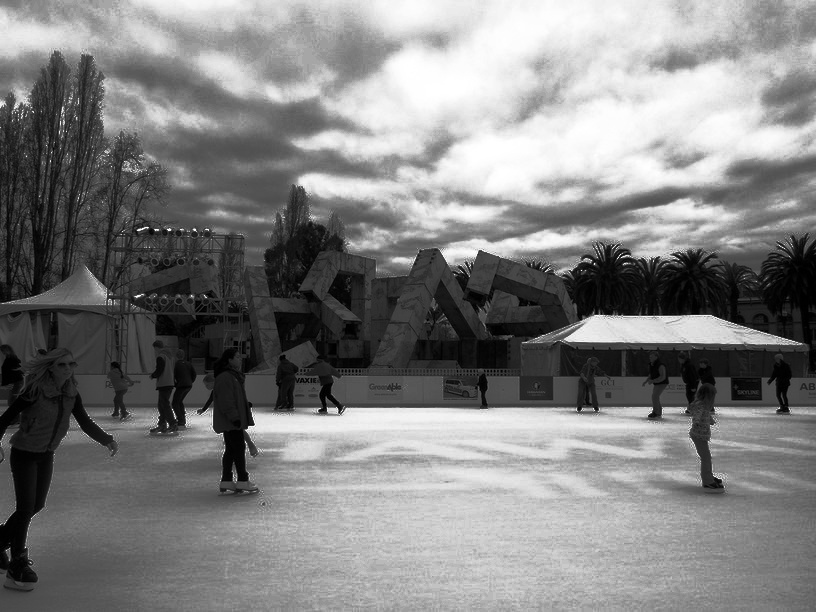
\includegraphics[width=\textwidth]{src.jpg}
        \caption{Imagem de referência}
        \label{fig:src}
    \end{subfigure}
    \qquad
    \begin{subfigure}[ht]{0.45\textwidth}
        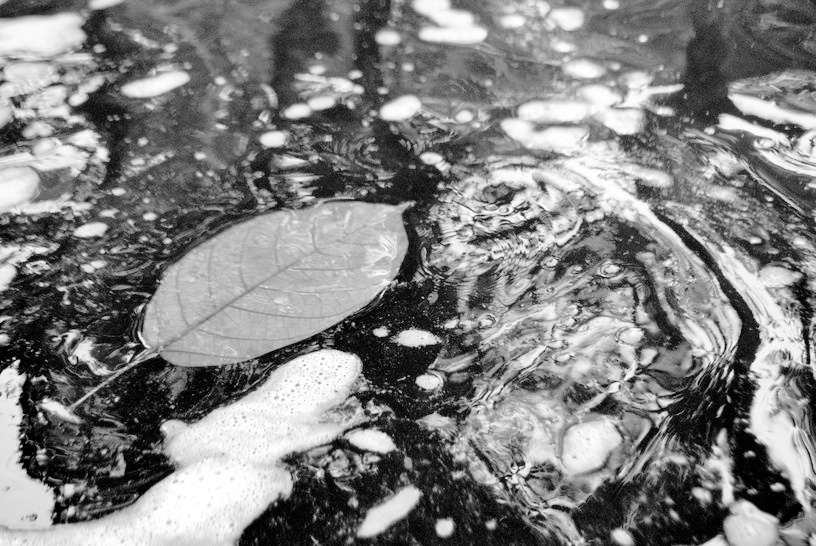
\includegraphics[width=\textwidth]{dst.jpg}
        \caption{Após casamento de histogramas}
        \label{fig:dst}
    \end{subfigure}
    \caption{Casamento de histogramas}
    \label{fig:cas_hist}
\end{figure}

\begin{thebibliography}{99}
    \bibitem{livro} GONZALEZ, Rafael C.; WOODS, Richard E.. \textbf{Digital Image Processing}. 3. ed. Upper Saddle River, NJ, EUA: Prentice-hall, 2006.
\bibitem{falcao} \texttt{http://www.ic.unicamp.br/afalcao/mo443/aula7.pdf}
\end{thebibliography}

\end{document}
